\documentclass{beamer}
\def\presentationtype{0}
\def\corsodilaurea{Ingegneria Informatica e dell'Automazione Industriale}
\def\insegnamento{Ottimizzazione}
\def\nolezione{8}
\def\titolo{Il metodo del simplesso -- Il ``tableau'' e l'operazione ``pivot''}
\def\noattivita{1}

\def\argomenti{Programmazione Lineare}
\def\obiettivilezione{Definire il ``tableau'' e l'operazione ``pivot'' per poter sviluppare metodo del simplesso primale}
\def\nucleotematico{Richiami}
\def\contenuto{Programmazione lineare}


\usepackage[italian]{babel}
%
% Hyperref info for PDF
%
\usepackage{hyperref}
\hypersetup{%
%pdfpagemode=FullScreen,
pdfpagemode=FullScreen,
pdfstartview=Fit,
pdfsubject={\argomenti},
pdfkeywords={\insegnamento,\titolo}
}

\definecolor{ecampus@engred}{RGB}{227,28,23}
\setbeamercolor{normal text}{fg=black,bg=}
\setbeamercolor{alerted text}{fg=red}
\setbeamercolor{example text}{fg=green!50!black}
\setbeamercolor{structure}{fg=ecampus@engred,bg=}
\usetheme{default}
\useinnertheme{rounded}%{circles}
\setbeamertemplate{blocks}[default]
\setbeamercolor{block title}{bg=}
\setbeamercolor{block body}{bg=}

\ifnum\presentationtype>0 {\setbeamertemplate{enumerate item}{Es. \nolezione.\presentationtype.\arabic{enumi})}} \fi

%\setbeamertemplate{frametitle continuation}[from second][(cont'd)]
\usefonttheme[stillsansseriftext,stillsansserifsmall]{serif}
\setbeamertemplate{headline}{%
\leavevmode%
   \hspace*{4.75cm}
   \scalebox{0.90}{%
    \begin{minipage}{\linewidth}%
      \tiny
 	\begin{tabular}{ll}
	  \\
% 	  \textcolor{gray}{Classe}					& \corsodilaurea\\
%	  \textcolor{gray}{Argomento:}					& \insegnamento\\
%	  \textcolor{gray}{Lezione n}:							& \nolezione \\
	  \textcolor{gray}{Titolo:}			& \titolo \\
	  \textcolor{gray}{Attivit\`a}:		& 	  \ifnum\presentationtype=0 {Lezione \nolezione} \else {Sessione di studio \nolezione.\presentationtype} \fi
	\end{tabular}%
    \end{minipage}%
   }%
}
\setbeamertemplate{footline}[text line]{%
  \begin{minipage}{\linewidth}%
    \hfill\insertpagenumber%
%    
    \begin{center}%
      \rule{\linewidth}{0.4pt}
    \end{center}
    \vspace*{-0.65cm}
    \begin{center}%
      \scalebox{0.55}{%
	\begin{minipage}{\linewidth}%
	  \begin{center}%
	    {\tiny
	    \copyright \ 2022 Gionata Massi - \color{blue}{\href{mailto:gionata.massi@savoiabenincasa.it}{gionata.massi@savoiabenincasa.it}}\\
	    \phantom{XXX}}
	  \end{center}
	\end{minipage}%
      }%
    \end{center}%
%
  \end{minipage}%
  }
\setbeamertemplate{navigation symbols}{}

%% Save up on ink for the 4-up handouts
\mode<handout>{%
  \pgfpagesuselayout{4 on 1}[a4paper, landscape, border shrink=10mm]
  \pgfpageslogicalpageoptions{1}{border code=\pgfstroke}
  \pgfpageslogicalpageoptions{2}{border code=\pgfstroke}
  \pgfpageslogicalpageoptions{3}{border code=\pgfstroke}
  \pgfpageslogicalpageoptions{4}{border code=\pgfstroke}
}

\mode<presentation>{\AtBeginSection{%
  \begin{frame}
    \frametitle{Piano della presentazione}
    \tableofcontents[currentsection]
  \end{frame}}
}

\usepackage{microtype}
\usepackage[utf8]{inputenc}
\usepackage[T1]{fontenc}
%\usepackage[osfss]{libertine}
\usepackage{palatino}
\usepackage[scaled=.77]{beramono}
\usepackage{booktabs}
% \usepackage{attachfile}

% Toglie l'enorme spazione prima di description
%\setbeamersize{description width=0pt}

\usepackage{tikz}
\usetikzlibrary{decorations,arrows,shapes,backgrounds,matrix,positioning}
\usepackage{multirow}
\usepackage{verbatim}
\usepackage{eurosym}
\usepackage{pgfpages}

\usepackage{zref-savepos}
\newcounter{restofframe}
\newsavebox{\restofframebox}
\newlength{\mylowermargin}
\setlength{\mylowermargin}{2pt}

\newenvironment{restofframe}{%
    \par%\centering
    \stepcounter{restofframe}%
    \zsavepos{restofframe-\arabic{restofframe}-begin}%
    \begin{lrbox}{\restofframebox}%
}{%
    \end{lrbox}%
    \setkeys{Gin}{keepaspectratio}%
    \raisebox{\dimexpr-\height+\ht\strutbox\relax}[0pt][0pt]{%
    \resizebox*{!}{\dimexpr\zposy{restofframe-\arabic{restofframe}-begin}sp-\zposy{restofframe-\arabic{restofframe}-end}sp-\mylowermargin\relax}%
        {\usebox{\restofframebox}}%
    }%
    \vskip0pt plus 1filll\relax
    \mbox{\zsavepos{restofframe-\arabic{restofframe}-end}}%
    \par
}

\title{\titolo}
\author{Gionata Massi}
\date{\today}

\setbeamercolor*{frametitle}{fg=black}
\setbeamercolor*{title}{fg=black}
\setbeamerfont{frametitle}{shape=\scshape,family=\rmfamily,size=\large,series=\bfseries}

\setbeamersize{}
\makeatletter
\newcommand\thefontsize[1]{{#1 The current font size is: \f@size pt\par}}
\makeatother

\tikzstyle{nicebox}=[draw=gray!100, fill=blue!10, very thick,
rounded corners, rectangle, inner sep=4pt, inner ysep=16pt]
\tikzstyle{niceboxtitle}=[draw=gray!100, fill=white, text=black,
rounded corners, very thick, rectangle]
\newcommand\nicebox[2]{
{\centering
\begin{tikzpicture}
\node [nicebox](box){
\begin{minipage}{0.95\textwidth}\centering
\begin{minipage}{0.95\textwidth}
#2
\end{minipage}\end{minipage}};
\node[niceboxtitle, right=10pt] at (box.north west)
{\small\textbf{#1}};
\end{tikzpicture}\par}
}

\tikzstyle{modelbox}=[draw=structure!100, fill=white!50, very thick,
rounded corners, rectangle, inner sep=4pt, inner ysep=16pt, text=blue!50!black]
\tikzstyle{modelboxtitle}=[draw=structure!100, fill=white!50, text=blue!50!black,
rounded corners, very thick, rectangle]
\newcommand\modelbox[2]{
{\centering
\begin{tikzpicture}
\node [modelbox](box){
\begin{minipage}{0.95\textwidth}\centering
\begin{minipage}{0.95\textwidth}
#2
\end{minipage}\end{minipage}};
\node[modelboxtitle, right=10pt] at (box.north west)
{\small\textbf{\mbox{#1}}};
\end{tikzpicture}\par}
}

% % %
% Tipi di sessioni di studio
% % %
\def\domande{Domande}
\def\approfondimenti{Approfondimenti}
\def\esercizi{Esercizi}
\def\esempi{Esempi svolti}
\def\relazioni{Relazioni}
\def\attivitapratica{Attivit\`a pratica}
% % %

\newcommand{\generatitolo}{ %
\begin{frame}[plain]
\pdfbookmark{\ifnum\presentationtype=0 {Lezione \nolezione} \else {Sessione di studio \nolezione.\presentationtype} \fi}{\ifnum\presentationtype=0 {Lezione \nolezione} \else {Sessione di studio \nolezione.\presentationtype} \fi}
\noindent\hspace*{3.715cm}
   \scalebox{0.90}{%
    \begin{minipage}{\linewidth}%
      \tiny
 	\begin{tabular}{ll}
	  \\
% 	  \textcolor{gray}{Classe}					& \corsodilaurea\\
%	  \textcolor{gray}{Argomento:}					& \insegnamento\\
%	  \textcolor{gray}{Lezione n}:							& \nolezione \\
	  \textcolor{gray}{Titolo:}			& \titolo \\
	  \textcolor{gray}{Attivit\`a}:		& 	  \ifnum\presentationtype=0 {Lezione \nolezione} \else {Sessione di studio \nolezione.\presentationtype} \fi
	\end{tabular}%
    \end{minipage}%
   }%
   
  \begin{center}
    \large{\textbf{\insegnamento}}
  \end{center}

  \vspace*{0.5cm}
  
  \begin{center}
    \huge{\titolo}
  \end{center}
  
  \begin{center}
	  \ifnum\presentationtype=0
	    {Lezione n$^{\circ}$ \nolezione}
	  \else
	    {Sessione di studio n$^{\circ}$ \nolezione .\presentationtype}
	  \fi
  \end{center}
  
  \vspace*{0.5cm}

  \begin{center}
    \large{\textsl{Gionata Massi}}\\
    \scriptsize\color{blue}{<\href{mailto:gionata.massi@savoiabenincasa.it}{gionata.massi@savoiabenincasa.it}>}
  \end{center}
  
  \newcounter{pageleft}
  \zsaveposy{pageleft}
  \vspace*{\dimexpr\zposy{pageleft}sp-1.67cm}

  \begin{minipage}{\linewidth}%
   \hfill\phantom{\insertpagenumber}%

  \begin{center}%
      \rule{\linewidth}{0.4pt}
    \end{center}
    
    \vspace*{-0.95cm}
    
    \begin{center}%
      \scalebox{0.55}{%
	\begin{minipage}{\linewidth}%
	  %\begin{center}%
	  %  \tiny
	  %  \copyright \ 2022 Gionata Massi - \color{blue}{\href{mailto:gionata.massi@savoiabenincasa.it}{gionata.massi@savoiabenincasa.it}}\\
	  %  \color{blue}{\href{mailto:gionata.massi@savoiabenincasa.it}{gionata.massi@savoiabenincasa.it}}\\
	  %  \phantom{XXX}
	  %\end{center}
	\end{minipage}%
      }%
    \end{center}%
     \phantom{XXX}
%
  \end{minipage}%

\end{frame}
}

\renewcommand{\vec}{\mathbf}
\newcommand{\matr}{\mathbf}

\uselanguage{italian}
\languagepath{italian}
\deftranslation[to=italian]{Theorem}{Teorema}
\deftranslation[to=italian]{theorem}{teorema}
\deftranslation[to=italian]{Definition}{Definizione}
\deftranslation[to=italian]{definition}{definizione}
\deftranslation[to=italian]{Corollary}{Corollario}
\deftranslation[to=italian]{corollary}{corollario}

\let\definition\relax
\let\enddefinition\relax

%\theoremstyle{example}
\newtheorem{definition}[theorem]{\translate{Definition}}

\def\fieldN{\mathbb{N}}
\def\fieldR{\mathbb{R}}
\def\fieldZ{\mathbb{Z}}

\def\matrA{\matr{A}}
\def\vecB{\vec{b}}
\def\vecC{\vec{c}}
\def\vecX{\vec{x}}

\usepackage{cancel}
\usepackage{bookmark}

% tkiz ball item
\newcommand*\circled[1]{\raisebox{2.5pt}{\tikz[baseline=(char.base)]{
            \node[circle,ball color=purple, shade, 
 color=white,inner sep=1.2pt] (char) {\tiny #1};}}}

% tkiz rounded item
\newcommand*\rounded[1]{\tikz[baseline=(char.base)]{
            \node[draw=none,ball color=purple, shade, 
 color=white, rounded corners=3.5pt, inner sep=2.5pt] (char) {\scriptsize #1};}}

 \usepackage{etoolbox}
\makeatletter
\apptocmd{\beamer@@frametitle}{\write\@auxout{\string\@writefile{frm}{\string\frametitleentry{\the\c@framenumber}{#1}{#2}}}}{}{}
\newcommand*{\frametitleentry}[3]{\@namedef{frametitleshort#1}{#2}\@namedef{frametitle#1}{#3}}
\AtEndDocument{\if@filesw\newwrite\tf@frm\immediate\openout\tf@frm\jobname.frm\relax\fi}
\@input{\jobname.frm}
\makeatother
 
%\usebackgroundtemplate{
\includegraphics[width=\paperwidth]{../img/sfondo_ecampus.png}}

\usepackage{listings}
% Extension for listings package
\lstdefinelanguage{ampl}{
  % See AMPL book (1993 edition), Appendix A
  morekeywords={%
    % Table A.1
    % Excluding symbols and "not X", where X (and not) are keywords
    if, then, else, or,  exists, forall,  and, in, within, 
    not, union, diff, symdiff, inter, cross, setof, by, 
    % Skipping: less,  sum, prod, min, max, div, mod,
    % Skipping built-in functions (Tables A-2 and A-3)
    % Section A.5 -- Declarations of model entities (subject to ->
    % subject, to)
    set, param, var, arc, minimize, maximize, subject, to, node,
    % Section A.6 -- Set declarations (not repeating set or within)
    dimen, default, card, ordered, by, reversed, circular,
    % Section A.7 -- Parameter declarations (not repeating in, default)
    param, binary, integer, symbolic, check, Infinity
    % Section A.8 -- Variable declarations
    var,  coeff, cover, obj,
    % Section A.13 -- Command language
    % Skipping most commands!
    include, model, data, let, objective, drop, restore, solve,
    solution, quit, end, option, reset, update, commands,
    % A.14 -- Imported functions
    function, pipe, 
    % A.17 synonyms for previously-defined keywords
    coef, difference, dimen, dimension, intersect, intersection, s.t., 
    % 
    % must be defined somewhere ...
    for, while, repeat, break,
    % NEW language features (http://www.ampl.com/NEW/newlang.html)
    % Grouped by page
    purge, problem, redeclare, xref,
    complements, 
    table, IN, OUT, INOUT, read, write, 
    expand,
    for, commands, repeat, until, while, break, continue,
  },
  sensitive=true,
  comment=[l]{\#},
  morecomment=[s]{/*}{*/},
  string=[b]",
  morestring=[b]',
}[keywords,comments,strings]

\definecolor{comment_c}{RGB}{60,128,49}
\definecolor{rowname_c}{RGB}{128,60,49}
\definecolor{reserved_c}{RGB}{49,60,128}

\lstset{
	language=ampl,%
	commentstyle=\color{comment_c},%
	backgroundcolor=\color{blue!15},%
    basicstyle=\small\ttfamily,%
    %emph={s.t.},emphstyle={\bfseries},%
    otherkeywords={s.t.},%
    numbers=left, numberstyle=\tiny, stepnumber=1, numbersep=5pt,%
}

\definecolor{col_set}{RGB}{128,0,0}
\definecolor{col_par}{RGB}{91,0,91}
\definecolor{col_idx}{RGB}{0,91,91}
\definecolor{col_var}{RGB}{0,0,128}

\def\insieme{%1}{\rm \textcolor{col_set}{%1}}}


\definecolor{comment_c}{RGB}{60,128,49}
\definecolor{rowname_c}{RGB}{128,60,49}
\definecolor{reserved_c}{RGB}{49,60,128}

\makeatletter

%%%%%%%%%%%%%%%%%%%%%%%%%%%%%% LyX specific LaTeX commands.
\newcommand{\noun}[1]{\textsc{#1}}

%%%%%%%%%%%%%%%%%%%%%%%%%%%%%% Textclass specific LaTeX commands.
 % this default might be overridden by plain title style
 \newcommand\makebeamertitle{\frame{\maketitle}}%
 \AtBeginDocument{
   \let\origtableofcontents=\tableofcontents
   \def\tableofcontents{\@ifnextchar[{\origtableofcontents}{\gobbletableofcontents}}
   \def\gobbletableofcontents#1{\origtableofcontents}
 }
 \long\def\lyxframe#1{\@lyxframe#1\@lyxframestop}%
 \def\@lyxframe{\@ifnextchar<{\@@lyxframe}{\@@lyxframe<*>}}%
 \def\@@lyxframe<#1>{\@ifnextchar[{\@@@lyxframe<#1>}{\@@@lyxframe<#1>[]}}
 \def\@@@lyxframe<#1>[{\@ifnextchar<{\@@@@@lyxframe<#1>[}{\@@@@lyxframe<#1>[<*>][}}
 \def\@@@@@lyxframe<#1>[#2]{\@ifnextchar[{\@@@@lyxframe<#1>[#2]}{\@@@@lyxframe<#1>[#2][]}}
 \long\def\@@@@lyxframe<#1>[#2][#3]#4\@lyxframestop#5\lyxframeend{%
   \frame<#1>[#2][#3]{\frametitle{#4}#5}}
 \def\lyxframeend{} % In case there is a superfluous frame end

\makeatother

\begin{document}

\generatitolo

\lyxframeend{}\section{Introduzione}


\lyxframeend{}\subsection{Motivazioni}


\lyxframeend{}\lyxframe{Perch\'e usare questo software?}
\begin{itemize}
\item La ``Ricerca Operativa'' \`e una disciplina \alert{applicata}.
\item La \alert{pratica} permette di comprendere meglio la teoria.

\item Possono essere indagati sul campo gli aspetti metodologici della Ricerca
Operativa, divenendo capaci di utilizzare tali conoscenze per interpretare,
formulare, descrivere e risolvere problemi.
\item Si possono condurre esperimenti ed analizzarne i dati e interpretarne i risultati.

\end{itemize}

\lyxframeend{}\subsection{Obiettivi}


\lyxframeend{}\lyxframe{Obiettivi}
\begin{itemize}
\item Usare strumenti software per: 

\begin{itemize}
\item la modellizzazione di problemi di Programmazione Matematica (PM);
\item la risoluzione dei PM;
\item l'analisi dei risultati;
\item l'implementazione di algoritmi ottimizzazione.

\end{itemize}
\item Uno strumento software che permette di conseguire tutti gli
	obiettivi \`e LINGO.
\end{itemize}

\lyxframeend{}\subsection{Metodologia}


\lyxframeend{}\lyxframe{Come opereremo?}

\begin{center}
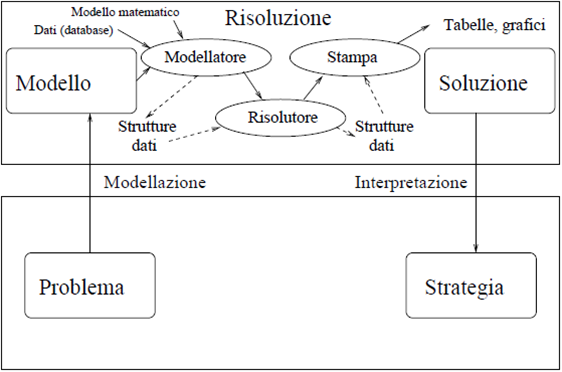
\includegraphics[width=0.7\textwidth]{img/approccio_modellistico}
\par\end{center}

\vspace*{-0.5cm}

\begin{center}
{\tiny Immagine tratta da ``\textit{Appunti sul
linguaggio di programmazione AMPL}'', R. Cordone,
M. Bruglieri, L. Liberti}
\end{center}


\lyxframeend{}\subsection{Strumenti}


\lyxframeend{}\lyxframe{Linguaggi di modellazione algebrica}

\begin{center}
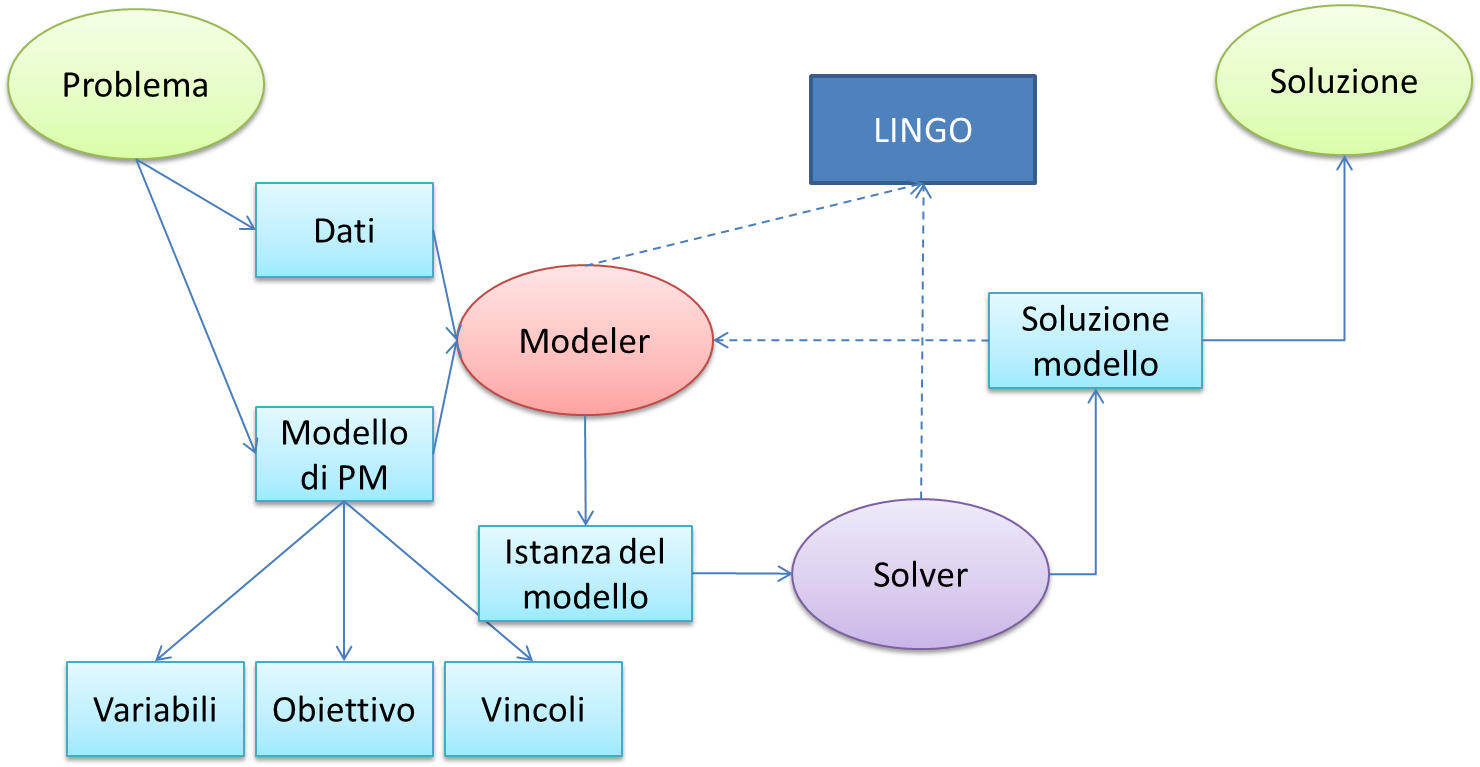
\includegraphics[width=0.8\textwidth]{img/linguaggi_mod_alg}
\par\end{center}


\lyxframeend{}\lyxframe{Alcuni linguaggi di modellazione algebrica}
\begin{itemize}
\item \href{https://www.minizinc.org/}{MiniZinc} (programmazione a vincoli)
\item AMPL, GAMS, AIMMS
\item XPRESS (impl.\ algoritmi avanzati, grafi)
\item OPL studio
\item OML (Microsoft Solver Foundation)
\item ZIMPL (suite gratuita per scopi non commerciali)
\item GMPL (sottoinsieme di AMPL, gratuito)
\end{itemize}

\lyxframeend{}\subsection{LINGO: istallazione}


\lyxframeend{}\lyxframe{LINGO: Installazione demo}
\begin{enumerate}
\item download (http://www.lindo.com/)

\begin{itemize}
\item men\`u Downloads voce Download LINGO
\end{itemize}
\item estrazione dei file dall'archivio/esecuzione dell'installer
\item avvio e scelta della \textquotedbl{}Demo version\textquotedbl{}

\begin{itemize}
\item limitazioni (versione per chi ha acquistato lo ''Hillier\&Lieberman''):

\begin{itemize}
\item 300 (500) variabili continue
\item 30 (50) variabili intere 
\item 50 (250)vincoli 
\end{itemize}
\end{itemize}
\end{enumerate}

\lyxframeend{}\subsection{LINGO: primi passi}


\lyxframeend{}\lyxframe{Risolutore interattivo}
%%\begin{itemize}
%%\item
L'ambiente LINGO, nel suo uso di base, permette di:

\begin{itemize}
\item introdurre un modello istanziato;
\item risolvere il modello;
\item analizzare la soluzione ottima;
\item effettuare l'analisi di post-ottimalit\`a:

\begin{itemize}
\item variabili duali;
\item intervalli di stabilit\`a.
\end{itemize}
\end{itemize}
%%\end{itemize}

\lyxframeend{}\lyxframe{[allowframebreaks]Introduzione di un PM istanziato}
\begin{block}{Variabili}
valori da determinare (non costanti) tramite cui misurare le prestazioni
\end{block}

\begin{block}{Funzione obiettivo (funzione delle variabili decisionali)}
Indice di prestazione del sistema da massimizzare (\noun{\structure{\noun{MAX =}} espressione};)
o minimizzare (\noun{\structure{\noun{MIN =}} espressione};)
\end{block}

\begin{block}{Vincoli}
insieme di restrizioni sui valori che possono essere assunti dalle variabili, a cui eventualmente pu\`o essere assegnato un
nome, ognuno nella forma:\\
\noun{<espressione> <operatore relazionale> <numero}>;
\end{block}

\lyxframeend{}\subsection{Esempio}\lyxframe{[allowframebreaks]Esempio: mix ottimo di produzione}

\begin{center}
$\begin{array}{rrrcr}
\max z= & 120\,x_{1} & +40\,x_{2}\\
 & 40\,x_{1} & +                    20\,x_{2} & \leq & 2200\\
 &  8\,x_{1} & +          \phantom{0}2\,x_{2} & \leq &  320\\
 &     x_{1} & +\phantom{0}\phantom{0}\,x_{2} & \leq &  100\\
 & x_{1} \geq 0, & x_{2} \geq 0
\end{array}$
\par\end{center}

%\begin{center}
%$\downarrow$
%\par\end{center}

\begin{exampleblock}
{Codice LINGO - Mix ottimo}

{\small
\textcolor{comment_c}{! Funzione obiettivo: massimo profitto;}\par

\textcolor{rowname_c}{{[}profit{]}} \textcolor{reserved_c}{MAX} = 120{*}x1 + 40{*}x2;\par

\textcolor{comment_c}{! Sistema dei vincoli;}\par

\textcolor{rowname_c}{{[}row\_mat{]}} 40{*}x1 + 20{*}x2 <= 2200;\par

\textcolor{rowname_c}{{[}labour{]}}~~~~~~~8{*}x1 +~~~2{*}x2 <=~~320;\par

\textcolor{rowname_c}{{[}market{]}}~~~~~~~~~x1 +~~~~~~~x2 <=~~100;\par
}
\end{exampleblock}

\lyxframeend{}\lyxframe{Risoluzione automatica del modello}
%%\begin{itemize}
%%\item
LINGO - Solve

\begin{description}
\item [{Model~Class}] Il tipo di modello riconosciuto dal risolutore
\item [{State}] Lo stato di uscita dell’algoritmo di risoluzione
\item [{Objective}] Il valore corrente della soluzione
\item [{Iterations}] Numero di iterazioni del risolutore.
\item [{…}]~
\item [{Elapsed~Runtime}] Tempo trascorso dall’inizio del processo di
soluzione. 
\end{description}
%%\end{itemize}

\lyxframeend{}\lyxframe{Screen shot formulazione e solution report}

\begin{center}
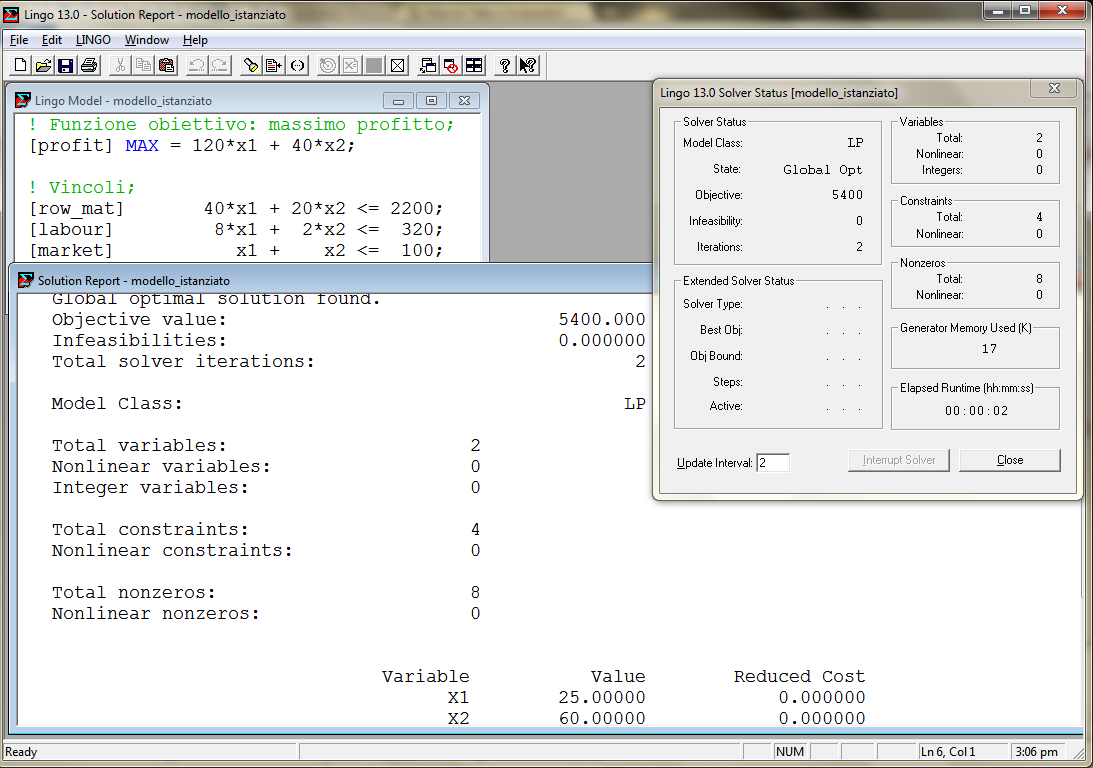
\includegraphics[height=0.85\textheight]{img/lingo_mod_istanz}
\par\end{center}


\lyxframeend{}

\begin{frame}[fragile]
\frametitle{Interpretazione dei risultati - modello}

%%\begin{itemize}
%%	\item
{Statistiche del modello (LINGO-Solve)}
%%\end{itemize}

\begin{verbatim}
Total solver iterations: 2
Model Class:            LP
Total variables:         2
Nonlinear variables:     0
Integer variables:       0
Total constraints:       4
Nonlinear constraints:   0
Total nonzeros:          8
Nonlinear nonzeros:      0
\end{verbatim}
\end{frame}

\begin{frame}[fragile]
\frametitle{Interpretazione dei risultati - sol.\ primale e duale}

%%\begin{itemize}
%%	\item
{Soluzione del modello (LINGO-Solve)}
%%\end{itemize}

\begin{verbatim}
Variable           Value       Reduced Cost
      X1        25.00000         0.000000
      X2        60.00000         0.000000

    Row    Slack or Surplus     Dual Price
PROFIT        5400.000           1.00000
ROW_MAT          0.000           1.00000
LABOUR           0.000          10.00000
MARKET          15.000           0.00000
\end{verbatim}
\end{frame}



\begin{frame}[fragile]
\frametitle{Interpretazione dei risultati}

%%\begin{itemize}
%%	\item
{Soluzione del modello (LINGO-Range) - stabilit\`a}
%%\end{itemize}

\small\begin{verbatim}
 Ranges in which the basis is unchanged:
                 Objective Coefficient Ranges:
                  Current     Allowable     Allowable
Variable      Coefficient      Increase      Decrease
      X1         120.0000      40.00000      40.00000
      X2         40.00000      20.00000      10.00000
                     Righthand Side Ranges:
                  Current     Allowable     Allowable
     Row              RHS      Increase      Decrease
 ROW_MAT         2200.000      200.0000      600.0000
  LABOUR         320.0000      120.0000      60.00000
  MARKET         100.0000      INFINITY      15.00000
\end{verbatim}
\end{frame}

\section{Sintassi di base}

\lyxframeend{}\lyxframe{[allowframebreaks]Sintassi di base}

\begin{block}{Commenti:}
iniziano con un punto esclamativo (\structure{!}) e terminano
al punto e virgola (\structure{;})
\end{block}

\begin{block}{Nomi di variabili:}
devono iniziare con un carattere alfabetico {[}A-Za-z{]} e non possono
contenere simboli di operatori o di punteggiatura. Case-insensitive.
\end{block}

\framebreak

\begin{block}{Funzione obiettivo:}
Un'espressione che lega variabili ed operatori aritmetici, preceduta
da un'eventuale denominazione fra parentesi quadre, preceduta da\\
\structure{MAX =} o \structure{MIN =}.\\
es: \structure{{[}}profit\structure{{]}} \structure{MAX $=$} \noun{espressione}
oppure\\
\structure{MIN $=$} \noun{espressione}
\end{block}

%\framebreak %\pagebreak<presentation>

\begin{block}{Vincoli:}
Un'espressione che lega variabili ed operatori aritmetici, preceduta
da un'eventuale denominazione fra parentesi quadre.\\
es: \structure{{[}}labour\structure{{]}} \noun{espressione}
\end{block}

\framebreak

\begin{block}{Operatori aritmetici:}
 in ordine di precedenza (alterato dalle parentesi
tonde)
\begin{itemize}
\item \structure{-} (negazione, unario), \structure{\textasciicircum{}},
\structure{{*}}, \structure{/}, \structure{+}, \structure{-} (sottrazione,
binario)
\end{itemize}
\end{block}

\begin{block}{Operatori relazionali:}
\begin{itemize}
\item \structure{$>=$}, \structure{$<=$}, \structure{$=$}
\end{itemize}
\end{block}

\begin{block}{Operatori logici:}
\begin{itemize}
\item \structure{\#NOT\#}, \structure{\#EQ\#}, \structure{\#NE\#}, \structure{\#GT\#},
\structure{\#GE\#}, \structure{\#LT\#}, \structure{\#LE\#}, \structure{\#AND\#},
\structure{\#OR\#}
\end{itemize}
\end{block}

\framebreak

\begin{block}{Dominio di una variabile:}
\begin{description}
\item [{@FREE~(\noun{variabile});}] \noun{variabile} , di default non
negativa, pu\`o assumere qualsiasi valore reale, positivo, negativo
o nullo.
\item [{@GIN(\noun{variabile});}] \noun{variabile} pu\`o assumere valori
interi non negativi. 
\item [{@BIN(\noun{variabile});}] \noun{variabile} deve assumere o il valore
0 o 1. 
\item [{@BND($lb$,~\noun{variabile},~$ub$);}] \noun{variabile} deve
essere compresa tra $lb$ e $ub$. 
\end{description}
\end{block}

\lyxframeend{}

\end{document}

\section{Uso del linguaggio di modellazione}


\lyxframeend{}\subsection{Costruzione del modello: insiemi e parametri}


\lyxframeend{}\lyxframe{Mix ottimo di produzione: modello scalare}
\begin{columns}%{}


\column{.50\textwidth}


\footnotesize{
\begin{description}
\item [{{\footnotesize $n$}}] {\footnotesize Numero dei prodotti}{\footnotesize \par}
\item [{{\footnotesize $m$}}] {\footnotesize Numero delle risorse }{\footnotesize \par}
\item [{{\footnotesize $a_{ij}$}}] {\footnotesize Assorbimento della risorsa
$i$ da un prodotto $j$ }{\footnotesize \par}
\item [{{\footnotesize $b_{i}$}}] {\footnotesize Disponibilit}\`a{\footnotesize{}
della risorsa $i$}{\footnotesize \par}
\item [{{\footnotesize $c_{j}$}}] {\footnotesize Profitto unitario prodotto
$j$}{\footnotesize \par}
\item [{{\footnotesize $x_{j}$}}] {\footnotesize Livello di produzione
prodotto $j$}{\footnotesize \par}
\end{description}

}


\column{.45\textwidth}


{\footnotesize $\begin{array}{cccc}
\max z= & {\displaystyle \sum_{j=1}^{n}}c_{j}\,x_{j}\\
	       & {\displaystyle \sum_{j=1}^{n}}a_{ij}\,x_{j} & \leq b_{i} & i=1,2,\ldots,m\\
 & x_{j}\geq0 &  & j=1,2,\ldots,n
\end{array}$}

\end{columns}%{}

\lyxframeend{}\lyxframe{Parametri e variabili del modello PL come vettori}

$\left.\mathbf{c}=\left[\begin{array}{c}
c_{1}\\
c_{2}\\
\vdots\\
c_{n}
\end{array}\right]\quad\mathbf{x}=\left[\begin{array}{c}
x_{1}\\
x_{2}\\
\vdots\\
x_{n}
\end{array}\right]\right\} $prodotti,$\left.\mathbf{b}=\left[\begin{array}{c}
b1\\
b_{2}\\
\vdots\\
b_{m}
\end{array}\right]\right\} $risorse,

$\left.\mathbf{A}=\left[\begin{array}{cccc}
a_{11} & a_{12} & \cdots & a_{1n}\\
a_{21} & a_{22} & \cdots & a_{2n}\\
\vdots & \vdots & \ddots & \vdots\\
a_{m1} & a_{m2} & \cdots & a_{mn}
\end{array}\right]\right\} $risorsa$\times$prodotto

\begin{center}
\fbox{%
$\begin{array}{rrl}
\max z = & \mathbf{c}^T \, \mathbf{x}\\
         & \mathbf{A}   \, \mathbf{x} & \leq \mathbf{b}\\
         & \mathbf{x}                 & \geq \mathbf{0}
\end{array}$%
}
\end{center}

\lyxframeend{}\lyxframe{Mix ottimo di produzione: modello basato su insiemi}
\begin{columns}%{}


\column{.50\textwidth}


\footnotesize{
\begin{description}
\item [{{\footnotesize $P$}}] {\footnotesize \alert{{\footnotesize Insieme}}
dei prodotti}{\footnotesize \par}
\item [{{\footnotesize $R$}}] {\footnotesize \alert{{\footnotesize Insieme}}
delle risorse }{\footnotesize \par}
\item [{{\footnotesize $a_{ij}$}}] {\footnotesize Assorbimento della risorsa
$i\in P$ da un prodotto $j\in R$ }{\footnotesize \par}
\item [{{\footnotesize $b_{i}$}}] {\footnotesize Disponibilit}\`a{\footnotesize{}
della risorsa $i\in R$}{\footnotesize \par}
\item [{{\footnotesize $c_{j}$}}] {\footnotesize Profitto unitario prodotto
$j\in P$}{\footnotesize \par}
\item [{{\footnotesize $x_{j}$}}] {\footnotesize Livello di produzione
prodotto $j\in P$}{\footnotesize \par}
\end{description}

}


\column{.45\textwidth}


\footnotesize{
$\begin{array}{cccc}
\max z= & {\displaystyle \sum_{\alert<2>{j\in P}}}c_{j}\,x_{j}\\
	       & {\displaystyle \sum_{\alert<2>{j\in P}}}a_{ij} \,x_{j} & \leq b_{i} & \alert<2>{i\in R}\\
  & x_{j}\geq0 &  & \alert<2>{j\in P}
\end{array}$
}

\end{columns}%{}

\lyxframeend{}\lyxframe{Confronto formulazioni scalari e basate su insiemi}
\begin{block}{Insiemi}
Gli indici sono stati fatti variare in un dominio, quello $P$ dei
prodotti e quello $R$ delle risorse

\begin{itemize}
\item $P=$\{$prod_{1},prod_{2}$\}
\item $R=\mbox{\{}row\_mat,labour,market$\}
\end{itemize}
\end{block}

\begin{block}{Attributi}
Gli elementi degli insiemi hanno degli attributi di interesse

\begin{itemize}
\item $P$: profitto per unit\`a prodotta ($c_{j}$), numero di prodotti
da realizzare ($x_{j}$)
\item $R$: disponibilit\`a della risorsa ($b_{i}$) 
\end{itemize}
\end{block}

\lyxframeend{}\subsection{Insiemi e attributi}


\lyxframeend{}\lyxframe{Insiemi e attributi in LINGO}

\begin{block}{Costrutto per la dichiarazione di insiemi primitivi}
Gli insiemi e i relativi attributi sono indicati come \\

\noun{insieme}: \noun{attributo}{[},\noun{ attributo}{]}{*};
\end{block}

\begin{exampleblock}{Esempio}
\structure{Prodotto: Profitto, X;}\\
\structure{Risorsa: Disponibilita;}
\end{exampleblock}

\lyxframeend{}\lyxframe{Insiemi derivati}

\begin{itemize}
\item Le quantit\`a $a_{ij}$ di risorsa assorbita dalla realizzazione
di un prodotto sono definite su tutte le coppie ordinate di una risorsa
e un prodotto.
\item Sono attributi del prodotto cartesiano di pi\`u insiemi e come tale
\`e detto insieme derivato.
\end{itemize}

\begin{block}{Costrutto per la dichiarazione di insiemi derivati}
 \noun{insieme\_derivato}(\noun{insieme}, \noun{insieme}{[}, \noun{insieme}{]}{*}):\\
\noun{attributo}{[}, \noun{attributo}{]}{*};
\end{block}

\begin{exampleblock}{Esempio}
\structure{RisorsaProdotto(Risorsa, Prodotto): Assorbimento;}
\end{exampleblock}

\lyxframeend{}\subsection{Combinazioni lineari e vincoli: iteratori}


\lyxframeend{}\lyxframe{Iterare sugli elementi di un insieme: somme}
\begin{columns}%{}


\column{4.5cm}


{\small Si vuole generare la combinazione lineare che moltiplica profitti
unitari e quantit\`a da produrre}{\small \par}
\begin{columns}%{}
\bigskip{}

\end{columns}%{}

{\Large
 \begin{equation*}
 {\displaystyle
 {\color{red!23!green!40!blue!70} \sum_{{\color{green!70!black} j} {\color{black} \in} {\color{red} P}}}}
    c_{\color{green!70!black} j}\,x_{{\color{green!70!black} j}} 
  \end{equation*}
}


\column{6.5cm}


{\small Si usa il costrutto

\structure{{\small @SUM(}} }\\
\ \ \  \noun{\small Insieme}{\small {[}(}\noun{\small indice}{\small {[},}\noun{\small indice}{\small {]}{*})\\
\ \ \ 
{[}| }\noun{\small condizioni}{\small {]]}\structure{{\small :}} }\noun{\small espressione}\\
{\small \structure{{\small );}}}{\small \par}
\begin{columns}%{}
\bigskip{}

\end{columns}%{}

{\small
  \structure{@SUM(} 
    {\color{red} Prodotto}({\color{green!70!black} j}):
      Profitto({\color{green!70!black} j}){*}X({\color{green!70!black} j})
   \structure{);}
}

\end{columns}%{}

\lyxframeend{}\lyxframe{Iterare sugli elementi di un insieme: cicli}
\begin{columns}%{}


\column{5cm}


{\small Si vogliono generare i vincoli sulle disponibilit\`a delle
risorse, uno per ogni risorsa $i$}\bigskip{}



{\Large  \begin{equation*}   {\displaystyle \sum_{j\in P}} a_{ij} \, x_{j} \leq b_{i} \quad {\color{green!70!black} i}\in {\color{red} R}  \end{equation*} }


\column{6cm}


{\small Si usa il costrutto

\structure{{\small @FOR(}} }\\
\ \ \ \noun{\small Insieme}{\small {[}(}\noun{\small indice}{\small {[},
}\noun{\small indice}{\small {]}{*})\\
\ \ \ {[}| }\noun{\small condizioni}{\small {]]}\structure{{\small :}}
}\noun{\small espressione}{\small\\
\structure{{\small );}}}{\small \par}
\begin{columns}%{}
\bigskip{}

\end{columns}%{}

\structure{@FOR(}\textcolor{red}{\ Risorsa}(\textcolor{green!70!black}{i}): $<$espressione$>$\structure{);}

\end{columns}%{}

\lyxframeend{}\subsection{Descrizione di un modello}


\lyxframeend{}\lyxframe{Descrizione di un modello}

\begin{block}{Linguaggio dichiarativo}
si dichiarano l'obiettivo e i dati con cui operare
\end{block}

\begin{block}{Algoritmi di soluzione gi\`a implementati}
la scelta dell'algoritmo di soluzione e la sua implementazione \`e
realizzata dal LINGO stesso
\end{block}

\begin{block}{Definizione di nuovi algoritmi}
si possono definire algoritmi più efficienti per risolvere classi di problemi,
in particolare definire sotto-problemi e implementare algoritmi di Column
Generation
\end{block}

\lyxframeend{}\lyxframe{Sezioni}
La dichiarazione del modello \`e divisa in sezioni, che si dichiarano con
 \structure{$<$Sezione$>$:} e terminano con \structure{$<$ENDSezione$>$}

\begin{description}
\item [{Model}] descrive il modello matematico
\item [{Sets}] descrive gli insiemi e relativi attributi
\item [{Data}] i parametri (istanza) del problema
\end{description}

Altre sezioni
\begin{description}
\item [{Init}] inserimento di soluzioni iniziali per prog.\ intera {[}mista{]}
e non lineare
\item [{Calc}] elaborazioni (per calcolare parametri derivati, per eseguire
istruzioni o descrivere algoritmi\ldots{})
\item [{Submodel}] un modello per un problema che pu\`o essere richiamato
nella sezione Calc
\end{description}

\lyxframeend{}\subsection{Implementazione del modello del MIX OTTIMO}


\lyxframeend{}\lyxframe{[allowframebreaks]Formulazione LINGO del mix ottimo}
\begin{exampleblock}
{Codice - 1 - Insiemi}

\textcolor{comment_c}{! Mix di produzione ottimo;}


\textcolor{comment_c}{! Sezione SETS;}

\structure{SETS}: 

\textcolor{comment_c}{! Gli insiemi primitivi;}

Risorsa: Disponibilita;

Prodotto: Profitto, X;\\

\textcolor{comment_c}{! Un insieme derivato;}

RisorsaProdotto(Risorsa, Prodotto): Assorbimento;

\structure{ENDSETS}
\end{exampleblock}
\framebreak %\pagebreak<presentation>
\begin{exampleblock}
{Codice - 2 - Formulazione}

\textcolor{comment_c}{! Il modello del problema di mix ottimo di produzione;}\\
\textcolor{comment_c}{! Massimizza il profitto totale;}

\textcolor{rowname_c}{{[}PROFITTO\_TOTALE{]}} \structure{MAX =} \structure{@SUM}( Prodotto(j):
Profitto(j){*}X(j));\\


\structure{@FOR}( Risorsa(i): \textcolor{comment_c}{! Per ogni risorsa i;}

~~~\textcolor{rowname_c}{{[}RISORSA\_{]}}

~~~\textcolor{comment_c}{! La quantit\`a utilizzata;}

~~~\structure{@SUM}( Prodotto(j): Assorbimento(i,j){*}X(j)) <= 

~~~~~Disponibilita(i); \textcolor{comment_c}{! deve essere <= di quella disponibile;}

); 
\end{exampleblock}
\framebreak %\pagebreak<presentation>
\begin{exampleblock}
{\small {Codice - 3 - Dati}}{\small \par}

{\small
\textcolor{comment_c}{! Sezione dati;}\\
\structure{{\small DATA}}:\\
\textcolor{comment_c}{! I nomi delle risorse e la loro disponibilita';}\\
Risorsa, Disponibilita =\\
~~~row\_mat 2200\\
~~~labour~~~~~~~320\\
~~~market~~~~~~100;\\
\textcolor{comment_c}{! I nomi dei prodotti e i loro profitti unitari;}\\
Prodotto, Profitto =\\
~~~prod1 120\\
~~~prod2~~~40;\\
\textcolor{comment_c}{! Matrice dei coefficienti tecnologici;}\\
Assorbimento = 40 20~~\textcolor{comment_c}{! Materie prime;}\\
~~~~~~~~~~~~~~~~~~~~~~~~~~~~8~~~2~~\textcolor{comment_c}{! Lavoro;}\\
~~~~~~~~~~~~~~~~~~~~~~~~~~~~1~~~1;~\textcolor{comment_c}{! Mercato;}\\
\structure{{\small ENDDATA}}
}
\end{exampleblock}

\lyxframeend{}\lyxframe{Comandi}

Selezionare del men\`u LINGO:

\begin{description}
\item [{Generate$\dasharrow$Display~model}] genera il modello istanziato
(\structure{@GEN();});
\item [{Generate$\dasharrow$Dual~model}] genera il modello del problema
duale associato (\structure{@GENDUAL();});
\item [{Solve}] determina una soluzione del modello (\structure{@SOLVE();});
\item [{Range}] determina gli intervalli di stabilit\`a;
\end{description}

\lyxframeend{}\lyxframe{Lettura dati da file}

LINGO permette di leggere dati da:

\begin{itemize}
\item file di testo nel formato LDT 

\begin{itemize}
\item \structure{@FILE( '\noun{filename}')}
\end{itemize}
\item fogli di calcolo Microsoft Excel

\begin{itemize}
\item \structure{@OLE( {[}'\noun{spreadsheet\_file}'{]} {[}, \noun{range\_name\_list}{]})}
\end{itemize}
\item basi di dati con ODBC

\begin{itemize}
\item \structure{@ODBC(\ldots{})}
\end{itemize}
\end{itemize}

\lyxframeend{}\lyxframe{Lettura dati da file di testo}

Il file della formulazione nella sezione dati dichiara il file esterno
da cui leggere 

\begin{itemize}
\item \noun{dato }= \structure{@FILE( '\noun{filename'})};
\end{itemize}

File di testo nel formato LDT

\begin{itemize}
\item Il file \noun{filename} contiene i dati

\begin{itemize}
\item i dati di uno stesso gruppo sono separati da caratteri di spazio
\item i dati di gruppo distinti sono separati simbolo end-of-record (\structure{\textasciitilde{}}).
\end{itemize}
\end{itemize}

\lyxframeend{}\lyxframe{Esempio lettura dati esterni}
\begin{exampleblock}
{\small Codice - Dichiarazione dati esterni}

{\small \textcolor{comment_c}{! Sezione dati;}

\structure{\small DATA}:

Risorsa = \structure{@FILE}('mix\_ottimo\_data.ldt');

Disponibilita = \structure{@FILE}('mix\_ottimo\_data.ldt');

Prodotto = \structure{@FILE}('mix\_ottimo\_data.ldt');

Profitto = \structure{@FILE}('mix\_ottimo\_data.ldt');

Assorbimento = \structure{@FILE}('mix\_ottimo\_data.ldt');

\structure{\small ENDDATA}}

\end{exampleblock}

\lyxframeend{}\lyxframe{Esempio lettura dati esterni}
\begin{exampleblock}
{\small File dati esterni - mix\_ottimo\_data.ldt}

{\small \textcolor{comment_c}{! I nomi delle risorse;}\\
row\_mat labour market \textasciitilde{}\\
\textcolor{comment_c}{! Le disponibilita' delle risorse;}\\
2200 320 100 \textasciitilde{}\\
\textcolor{comment_c}{! I nomi dei prodotti;}\\
prod1 prod2 \textasciitilde{}\\
\textcolor{comment_c}{! I profitti unitari dei prodotti;}\\
120 40 \textasciitilde{}\\
\textcolor{comment_c}{! Matrice dei coefficienti tecnologici;}\\
40 20 \textcolor{comment_c}{! Materie prime;}\\
~~8~~ 2 \textcolor{comment_c}{! Lavoro;}\\
~~1~~ 1 \textcolor{comment_c}{! Mercato; }
}
\end{exampleblock}

\lyxframeend{}

\lyxframeend{}\subsection{Per approfondire}


\lyxframeend{}\lyxframe{Per approfondire}

\beamertemplatebookbibitems
\begin{thebibliography}{References}
\bibitem{HillierLiebermanS1C3}F.S. Hillier, G. J. Lieberman.\newblock
\textit{Ricerca Operativa}.\newblock Supplemento 1 al Capitolo 3:
The LINGO modeling language. McGraw Hill, 2010.

\bibitem{Schrage2006} L. Schrage.\newblock \emph{Optimization Modeling
with LINGO.} \newblock LINDO Systems, Inc., 2006

\bibitem{LingoUserManual} LINDO Systems Inc.\newblock \emph{LINGO
User's guide.} \newblock LINDO Systems, Inc., 2011

\end{thebibliography}

\lyxframeend{}


\end{document}
